\RequirePackage{fix-cm}
\documentclass[tikz,border=3pt]{standalone}
\usepackage{amsmath,amssymb}
\usepackage{helvet}
\renewcommand{\familydefault}{\sfdefault}
\usetikzlibrary{arrows.meta,calc,positioning}
\definecolor{ink}{HTML}{35404B}
\definecolor{blue}{HTML}{466F9C}
\definecolor{bluelite}{HTML}{EFF5FB}
\definecolor{green}{HTML}{277F68}
\definecolor{greenlite}{HTML}{EAF7F0}
\definecolor{purple}{HTML}{8A6CAE}
\definecolor{purplelite}{HTML}{F3EFF9}
\definecolor{pinklite}{HTML}{FCEFF4}
\definecolor{gold}{HTML}{AC772A}
\definecolor{goldlite}{HTML}{FBF4E8}
\definecolor{graylite}{HTML}{F0F2F4}
\definecolor{coral}{HTML}{CD7A61}
\begin{document}
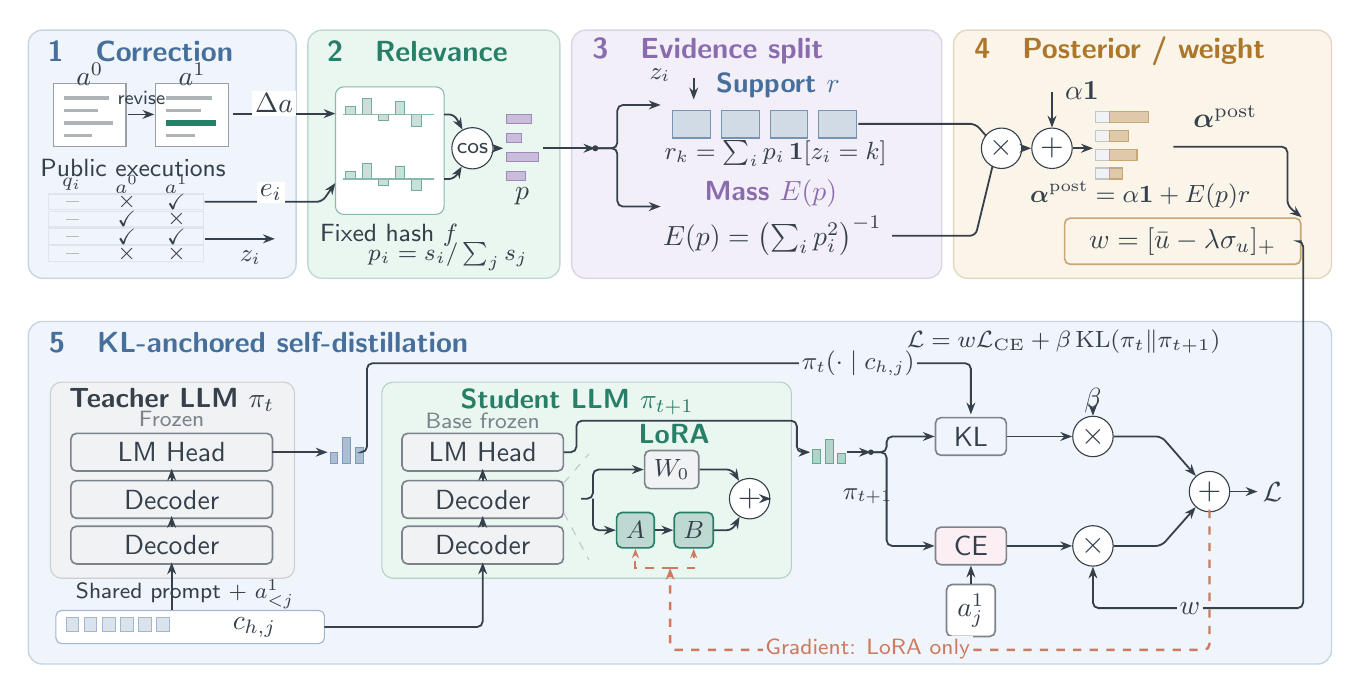
\begin{tikzpicture}[x=1cm,y=1cm,font=\fontsize{10}{11}\selectfont,text=ink,
 arr/.style={-{Stealth[length=1.5mm]},draw=ink,line width=.65pt,rounded corners=2pt},
 border/.style={rounded corners=5pt,line width=.5pt,draw=blue!30,fill=bluelite},
 block/.style={rounded corners=2pt,draw=ink!65,line width=.6pt,fill=graylite,align=center,minimum height=.40cm},
 sum/.style={circle,draw=ink,fill=white,inner sep=1.2pt,font=\fontsize{11}{11}\selectfont},
 head/.style={font=\bfseries\fontsize{10.5}{12}\selectfont,anchor=west}]
% Four evidence-processing regions, with only short visible labels.
\draw[border] (0,0) rectangle (3.4,-3.15);
\draw[border,draw=green!30,fill=greenlite] (3.55,0) rectangle (6.75,-3.15);
\draw[border,draw=purple!30,fill=purplelite] (6.9,0) rectangle (11.6,-3.15);
\draw[border,draw=gold!30,fill=goldlite] (11.75,0) rectangle (16.55,-3.15);
\node[head,text=blue] at (.12,-.27) {1\quad Correction};
\node[head,text=green] at (3.67,-.27) {2\quad Relevance};
\node[head,text=purple] at (7.04,-.27) {3\quad Evidence split};
\node[head,text=gold] at (11.89,-.27) {4\quad Posterior / weight};
% Source pair: abstract code lines, never a purported real program.
\foreach \xx/\lab in {.32/a^0,1.62/a^1}{
 \draw[fill=white,draw=ink!50] (\xx,-.68) rectangle ++(.92,-.80);
 \node at (\xx+.46,-.56) {$\lab$};
 \foreach \yy/\ww in {-.86/.58,-1.02/.44,-1.18/.63,-1.34/.36}
   \draw[draw=ink!40,line width=1.3pt] (\xx+.13,\yy)--++(\ww,0);
}
\draw[green,line width=2pt] (1.75,-1.18)--++(.63,0);
\draw[arr] (1.27,-1.07)--node[above,font=\scriptsize]{revise}(1.60,-1.07);
\node[font=\fontsize{9}{10}\selectfont] at (1.33,-1.75) {Public executions};
\node[font=\scriptsize] at (.55,-1.96) {$q_i$};
\node[font=\scriptsize] at (1.25,-1.96) {$a^0$};
\node[font=\scriptsize] at (1.88,-1.96) {$a^1$};
\foreach \yy/\a/\b in {-2.18/\times/\checkmark,-2.40/\checkmark/\times,-2.62/\checkmark/\checkmark,-2.84/\times/\times}{
 \draw[draw=blue!18] (.26,\yy+.10) rectangle (2.22,\yy-.10);
 \draw[ink!35] (.48,\yy)--(.64,\yy);
 \node[font=\fontsize{8}{9}\selectfont] at (1.25,\yy) {$\a$};
 \node[font=\fontsize{8}{9}\selectfont] at (1.88,\yy) {$\b$};
}
\draw[arr] (2.60,-1.06)--(3.90,-1.06);\node[fill=white,inner sep=1pt] at (3.12,-.93) {$\Delta a$};
\draw[arr] (2.24,-2.18)--(3.73,-2.18)--(3.90,-1.94);\node[fill=white,inner sep=1pt] at (3.08,-2.06) {$e_i$};
\draw[arr] (2.24,-2.65)--(3.13,-2.65);\node[font=\small] at (2.82,-2.89) {$z_i$};
% Fixed feature hashing, cosine scoring, normalized p.
\draw[fill=white,draw=green!55,rounded corners=3pt] (3.90,-.72) rectangle (5.28,-2.34);
\foreach \y in {-1.07,-1.89}{
 \foreach \k/\h in {0/.10,1/.20,2/-.08,3/.16,4/-.15}
  \draw[fill=green!25,draw=green!65,line width=.3pt] (4.03+.21*\k,\y) rectangle ++(.12,\h);
 \draw[green!55] (3.99,\y)--(5.15,\y);
}
\node[font=\fontsize{9}{10}\selectfont] at (4.58,-2.60) {Fixed hash $f$};
\node[sum,font=\fontsize{8}{9}\selectfont] (cos) at (5.64,-1.50) {cos};
\draw[arr] (5.28,-1.07)--(5.41,-1.07)--(cos);
\draw[arr] (5.28,-1.89)--(5.41,-1.89)--(cos);
\draw[arr] (cos)--(6.03,-1.50);
\foreach \yy/\w in {-1.07/.32,-1.31/.19,-1.55/.41,-1.79/.24}
 \draw[fill=purple!45,draw=purple!80] (6.07,\yy) rectangle ++(\w,-.12);
\node at (6.27,-2.11) {$p$};
\node[font=\fontsize{8.5}{10}\selectfont] at (5.33,-2.88) {$p_i=s_i/\sum_j s_j$};
% True parallel split. z_i is a named matched connector to avoid crossing.
\draw[arr] (6.54,-1.50)--(7.20,-1.50);\fill[ink] (7.2,-1.50) circle (1.1pt);
\draw[arr] (7.20,-1.50)--(7.48,-1.50)--(7.48,-.95)--(8.03,-.95);
\draw[arr] (7.20,-1.50)--(7.48,-1.50)--(7.48,-2.24)--(8.03,-2.24);
\draw[arr] (8.45,-.61)--(8.45,-.88);\node[font=\small] at (8.02,-.57) {$z_i$};
\node[font=\bfseries,text=blue] at (9.52,-.70) {Support $r$};
\foreach \k in {0,1,2,3}
 \draw[fill=blue!25,draw=blue!75] (8.18+.62*\k,-1.02) rectangle ++(.48,-.35);
\node[font=\fontsize{9}{10}\selectfont] at (9.49,-1.57) {$r_k=\sum_i p_i\,\mathbf{1}[z_i=k]$};
\node[text=purple,font=\bfseries] at (9.43,-2.07) {Mass $E(p)$};
\node[font=\fontsize{10}{11}\selectfont] at (9.45,-2.61) {$E(p)=\bigl(\sum_i p_i^2\bigr)^{-1}$};
\draw[arr] (10.54,-1.19)--(12.03,-1.19)--(12.30,-1.50);
\draw[arr] (10.97,-2.61)--(12.03,-2.61)--(12.30,-1.50);
\node[sum] (mult) at (12.36,-1.50) {$\times$};
\node[sum] (prioradd) at (13.00,-1.50) {$+$};\draw[arr] (mult)--(prioradd);
\draw[arr] (13.00,-.78)--(prioradd);\node at (13.38,-.77) {$\alpha\mathbf{1}$};
\draw[arr] (prioradd)--(13.52,-1.50);
\foreach \yy/\ww in {-1.03/.50,-1.27/.24,-1.51/.35,-1.75/.16}{
 \draw[fill=graylite,draw=ink!30] (13.55,\yy) rectangle ++(.18,-.14);
 \draw[fill=gold!40,draw=gold!65] (13.73,\yy) rectangle ++(\ww,-.14);
}
\node at (15.20,-1.10) {$\boldsymbol\alpha^{\rm post}$};
\node[font=\fontsize{9}{10}\selectfont] at (14.12,-2.09) {$\boldsymbol\alpha^{\rm post}=\alpha\mathbf{1}+E(p)r$};
\node[block,fill=goldlite,draw=gold!65,minimum width=3.00cm] (weight) at (14.66,-2.68) {$w=[\bar u-\lambda\sigma_u]_+$};
\draw[arr] (14.54,-1.48)--(15.99,-1.48)--(15.99,-2.23)--(weight.north east);
% Training band.
\draw[border] (0,-3.70) rectangle (16.55,-8.05);
\node[head,text=blue] at (.14,-3.96) {5\quad KL-anchored self-distillation};
% Teacher.
\draw[rounded corners=4pt,fill=graylite,draw=ink!25] (.28,-4.47) rectangle (3.38,-6.96);
\node[font=\bfseries] at (1.82,-4.70) {Teacher LLM $\pi_t$};
\node[font=\fontsize{8}{9}\selectfont,text=ink!65] at (1.82,-4.94) {Frozen};
\foreach \yy/\txt in {-5.36/LM Head,-5.96/Decoder,-6.54/Decoder}{
 \node[block,minimum width=2.56cm] at (1.82,\yy) {\txt};
}
\draw[arr] (1.82,-6.31)--(1.82,-6.17);\draw[arr] (1.82,-5.73)--(1.82,-5.57);
% Student. Green is restricted to the trainable low-rank path.
\draw[rounded corners=4pt,fill=greenlite,draw=green!35] (4.49,-4.47) rectangle (9.69,-6.96);
\node[font=\bfseries,text=green] at (6.97,-4.72) {Student LLM $\pi_{t+1}$};
\foreach \yy/\txt in {-5.36/LM Head,-5.96/Decoder,-6.54/Decoder}{
 \node[block,minimum width=2.05cm] at (5.77,\yy) {\txt};
}
\draw[arr] (5.77,-6.31)--(5.77,-6.17);\draw[arr] (5.77,-5.73)--(5.77,-5.57);
\node[font=\fontsize{8}{9}\selectfont,text=ink!65] at (5.77,-4.96) {Base frozen};
\node[font=\bfseries,text=green] at (8.20,-5.13) {LoRA};
\draw[ink!30,dashed,line width=.4pt] (6.80,-5.75)--(7.12,-5.38);
\draw[ink!30,dashed,line width=.4pt] (6.80,-6.13)--(7.12,-6.73);
% Representative linear projection: x -> W0 or A -> B -> sum.
\node[block,minimum width=.65cm,minimum height=.38cm,font=\small] (w0) at (8.17,-5.58) {$W_0$};
\node[block,fill=green!30,draw=green,minimum width=.42cm,minimum height=.45cm,font=\small] (la) at (7.71,-6.35) {$A$};
\node[block,fill=green!30,draw=green,minimum width=.42cm,minimum height=.45cm,font=\small] (lb) at (8.45,-6.35) {$B$};
\node[sum] (ladd) at (9.16,-5.95) {$+$};
\draw[arr] (7.02,-5.95)--(7.17,-5.95)--(7.17,-5.58)--(w0);
\draw[arr] (7.17,-5.95)--(7.17,-6.35)--(la);\draw[arr] (la)--(lb);
\draw[arr] (w0)--(8.94,-5.58)--(ladd);\draw[arr] (lb)--(8.94,-6.35)--(ladd);
\draw[arr] (ladd)--(9.43,-5.95);
% Shared prefixes enter BOTH model bottoms. No evidence / teacher output goes into student input.
\draw[rounded corners=2pt,fill=white,draw=blue!50] (.35,-7.37) rectangle (3.76,-7.79);
\foreach \i in {0,...,5}\draw[fill=blue!20,draw=blue!50,line width=.3pt] (.48+.23*\i,-7.46) rectangle ++(.16,-.18);
\node at (2.87,-7.58) {$c_{h,j}$};
\draw[arr] (1.82,-7.37)--(1.82,-6.76);
\draw[arr] (3.76,-7.58)--(5.77,-7.58)--(5.77,-6.76);
\node[font=\fontsize{8}{9}\selectfont] at (1.99,-7.16) {Shared prompt + $a^1_{<j}$};
% Two output distributions go to KL, student also to CE.
\draw[arr] (3.10,-5.36)--(3.80,-5.36);
\foreach \x/\h in {3.83/.14,3.99/.33,4.15/.20}\draw[fill=blue!45,draw=blue!70,line width=.3pt] (\x,-5.50) rectangle ++(.10,\h);
\draw[arr] (4.24,-5.36)--(4.30,-5.36)--(4.30,-4.23)--(11.97,-4.23)--(11.97,-4.88);
\node[font=\small,fill=bluelite,inner sep=1pt] at (10.54,-4.23) {$\pi_t(\cdot\mid c_{h,j})$};
\draw[arr] (6.80,-5.36)--(6.96,-5.36)--(6.96,-4.96)--(9.76,-4.96)--(9.76,-5.36)--(9.93,-5.36);
\foreach \x/\h in {9.96/.18,10.12/.30,10.28/.12}\draw[fill=green!35,draw=green!70,line width=.3pt] (\x,-5.50) rectangle ++(.10,\h);
\coordinate (split) at (10.70,-5.36);\draw[arr] (10.40,-5.36)--(split);\fill[ink] (split) circle (1pt);
\node[block,fill=bluelite,minimum width=.90cm] (kl) at (11.97,-5.16) {KL};
\node[block,fill=pinklite,minimum width=.90cm] (ce) at (11.97,-6.55) {CE};
\draw[arr] (split)--(10.90,-5.36)--(10.90,-5.16)--(kl);
\draw[arr] (split)--(10.90,-5.36)--(10.90,-6.55)--(ce);
\node[font=\small] at (10.66,-5.92) {$\pi_{t+1}$};
\node[block,fill=white,minimum width=.62cm] (target) at (11.97,-7.37) {$a^1_j$};\draw[arr] (target)--(ce);
% CE has w. KL has beta. Sum once, in the correct direction.
\node[sum] (kw) at (13.52,-5.16) {$\times$};\node[sum] (cw) at (13.52,-6.55) {$\times$};
\draw[arr] (kl)--(kw);\draw[arr] (ce)--(cw);
\node at (13.52,-4.71) {$\beta$};\draw[arr] (13.52,-4.87)--(kw.north);
\draw[arr] (weight.east)--(16.19,-2.68)--(16.19,-7.34)--(13.52,-7.34)--(cw);
\node[fill=bluelite,inner sep=1pt] at (14.75,-7.34) {$w$};
\node[sum] (loss) at (15.00,-5.86) {$+$};
\draw[arr] (kw)--(14.39,-5.16)--(loss);\draw[arr] (cw)--(14.39,-6.55)--(loss);
\draw[arr] (loss)--(15.61,-5.86);\node at (15.80,-5.86) {$\mathcal L$};
\node[font=\fontsize{8.5}{10}\selectfont] at (13.15,-3.96) {$\mathcal L=w\mathcal L_{\rm CE}+\beta\,\mathrm{KL}(\pi_t\Vert\pi_{t+1})$};
% Gradients flow only to trainable A and B.
\draw[-{Stealth[length=1.5mm]},coral,dashed,line width=.85pt,rounded corners=2pt]
 (15.00,-6.09)--(15.00,-7.87)--(8.15,-7.87)--(8.15,-6.83);
\draw[-{Stealth[length=1.2mm]},coral,dashed,line width=.75pt] (8.15,-6.83)--(7.71,-6.83)--(la.south);
\draw[-{Stealth[length=1.2mm]},coral,dashed,line width=.75pt] (8.15,-6.83)--(8.45,-6.83)--(lb.south);
\node[font=\fontsize{8}{9}\selectfont,text=coral,fill=bluelite,inner sep=1pt] at (10.66,-7.86) {Gradient: LoRA only};
\end{tikzpicture}
\end{document}
